\documentclass[english, 11pt]{article}\usepackage[]{graphicx}\usepackage[]{color}
%% maxwidth is the original width if it is less than linewidth
%% otherwise use linewidth (to make sure the graphics do not exceed the margin)
\makeatletter
\def\maxwidth{ %
  \ifdim\Gin@nat@width>\linewidth
    \linewidth
  \else
    \Gin@nat@width
  \fi
}
\makeatother

\definecolor{fgcolor}{rgb}{0.345, 0.345, 0.345}
\newcommand{\hlnum}[1]{\textcolor[rgb]{0.686,0.059,0.569}{#1}}%
\newcommand{\hlstr}[1]{\textcolor[rgb]{0.192,0.494,0.8}{#1}}%
\newcommand{\hlcom}[1]{\textcolor[rgb]{0.678,0.584,0.686}{\textit{#1}}}%
\newcommand{\hlopt}[1]{\textcolor[rgb]{0,0,0}{#1}}%
\newcommand{\hlstd}[1]{\textcolor[rgb]{0.345,0.345,0.345}{#1}}%
\newcommand{\hlkwa}[1]{\textcolor[rgb]{0.161,0.373,0.58}{\textbf{#1}}}%
\newcommand{\hlkwb}[1]{\textcolor[rgb]{0.69,0.353,0.396}{#1}}%
\newcommand{\hlkwc}[1]{\textcolor[rgb]{0.333,0.667,0.333}{#1}}%
\newcommand{\hlkwd}[1]{\textcolor[rgb]{0.737,0.353,0.396}{\textbf{#1}}}%
\let\hlipl\hlkwb

\usepackage{framed}
\makeatletter
\newenvironment{kframe}{%
 \def\at@end@of@kframe{}%
 \ifinner\ifhmode%
  \def\at@end@of@kframe{\end{minipage}}%
  \begin{minipage}{\columnwidth}%
 \fi\fi%
 \def\FrameCommand##1{\hskip\@totalleftmargin \hskip-\fboxsep
 \colorbox{shadecolor}{##1}\hskip-\fboxsep
     % There is no \\@totalrightmargin, so:
     \hskip-\linewidth \hskip-\@totalleftmargin \hskip\columnwidth}%
 \MakeFramed {\advance\hsize-\width
   \@totalleftmargin\z@ \linewidth\hsize
   \@setminipage}}%
 {\par\unskip\endMakeFramed%
 \at@end@of@kframe}
\makeatother

\definecolor{shadecolor}{rgb}{.97, .97, .97}
\definecolor{messagecolor}{rgb}{0, 0, 0}
\definecolor{warningcolor}{rgb}{1, 0, 1}
\definecolor{errorcolor}{rgb}{1, 0, 0}
\newenvironment{knitrout}{}{} % an empty environment to be redefined in TeX

\usepackage{alltt}
\usepackage{haziq_article}
\IfFileExists{upquote.sty}{\usepackage{upquote}}{}
\begin{document}

% This is the main code chunk to configure patchDVI using knitr and multi-file
% projects.


%%%%%%%%%%%%%%%%%%%%%%%%%%%%%%%%%%%%%%%%%%%%%%%%%%%%%%%%%%%%%%%%%%%%%%%%%%%%%%%%
%%% TITLE %%%%%%%%%%%%%%%%%%%%%%%%%%%%%%%%%%%%%%%%%%%%%%%%%%%%%%%%%%%%%%%%%%%%%%
%%%%%%%%%%%%%%%%%%%%%%%%%%%%%%%%%%%%%%%%%%%%%%%%%%%%%%%%%%%%%%%%%%%%%%%%%%%%%%%%
\pagenumbering{arabic}
\title{An apt title}
\author{	Haziq Jamil\\
			\normalsize{\it{Department of Statistics}}\\
			\normalsize{\it{London School of Economics \& Political Science}}
}
\date{\normalsize\today}
\maketitle
%{\let\newpage\relax\maketitle}  % if need some text before the title use this

%%%%%%%%%%%%%%%%%%%%%%%%%%%%%%%%%%%%%%%%%%%%%%%%%%%%%%%%%%%%%%%%%%%%%%%%%%%%%%%%
%%% ABSTRACT %%%%%%%%%%%%%%%%%%%%%%%%%%%%%%%%%%%%%%%%%%%%%%%%%%%%%%%%%%%%%%%%%%%
%%%%%%%%%%%%%%%%%%%%%%%%%%%%%%%%%%%%%%%%%%%%%%%%%%%%%%%%%%%%%%%%%%%%%%%%%%%%%%%%
\begin{abstract}
This is an abstract. \lipsum[1]
\end{abstract}

%%%%%%%%%%%%%%%%%%%%%%%%%%%%%%%%%%%%%%%%%%%%%%%%%%%%%%%%%%%%%%%%%%%%%%%%%%%%%%%%
%%% KEYWORDS %%%%%%%%%%%%%%%%%%%%%%%%%%%%%%%%%%%%%%%%%%%%%%%%%%%%%%%%%%%%%%%%%%%
%%%%%%%%%%%%%%%%%%%%%%%%%%%%%%%%%%%%%%%%%%%%%%%%%%%%%%%%%%%%%%%%%%%%%%%%%%%%%%%%
{\noindent\textbf{Keywords:} 
	some, keywords, go, here
}

%%%%%%%%%%%%%%%%%%%%%%%%%%%%%%%%%%%%%%%%%%%%%%%%%%%%%%%%%%%%%%%%%%%%%%%%%%%%%%%%
%%% BODY %%%%%%%%%%%%%%%%%%%%%%%%%%%%%%%%%%%%%%%%%%%%%%%%%%%%%%%%%%%%%%%%%%%%%%%
%%%%%%%%%%%%%%%%%%%%%%%%%%%%%%%%%%%%%%%%%%%%%%%%%%%%%%%%%%%%%%%%%%%%%%%%%%%%%%%%
\section{Introduction}
%\documentclass[class=article, crop=false]{standalone}
%\ifstandalone
%\usepackage{haziq_article}
%\fi
%
%\begin{document}

Following \cite{jamil2017},	\lipsum[2-3]

%%%%%%%%%%%%%%%%%%%%%%%%%%%%%%%%%%%%%%%%%%%%%%%%%%%%%%%%%%%%%%%%%%%%%%%%
%%% REFERENCES %%%%%%%%%%%%%%%%%%%%%%%%%%%%%%%%%%%%%%%%%%%%%%%%%%%%%%%%%
%%%%%%%%%%%%%%%%%%%%%%%%%%%%%%%%%%%%%%%%%%%%%%%%%%%%%%%%%%%%%%%%%%%%%%%%
%\ifstandalone
%%\nocite{*}
%\bibliographystyle{apalike}
%\bibliography{haziq}
%\fi
%
%\end{document}

















\section{Body}
%\documentclass[class=article, crop=false]{standalone}
%\ifstandalone
%\usepackage{haziq_article}
%\fi
%\begin{document}

\lipsum[4]

\subsection{One such subsection}

\lipsum[5-8]

\subsection{And another subsection}

We have seen in \cite{bergsma2017}, \lipsum[9]

%%%%%%%%%%%%%%%%%%%%%%%%%%%%%%%%%%%%%%%%%%%%%%%%%%%%%%%%%%%%%%%%%%%%%%%%
%%% REFERENCES %%%%%%%%%%%%%%%%%%%%%%%%%%%%%%%%%%%%%%%%%%%%%%%%%%%%%%%%%
%%%%%%%%%%%%%%%%%%%%%%%%%%%%%%%%%%%%%%%%%%%%%%%%%%%%%%%%%%%%%%%%%%%%%%%%
%\ifstandalone
%%\nocite{*}
%\bibliographystyle{apalike}
%\nobibliography{haziq}
%\fi
%
%\end{document}

















\section{R code}
%\import{}{03-rnw}
%\subimport{}{03-rnw}
%%!TEX root = main.Rnw
%\documentclass[class=article, crop=false]{standalone}
%\ifstandalone
%\usepackage{haziq_article}
%\fi
%\begin{document}



We can include some R code here. Hello

\begin{knitrout}
\definecolor{shadecolor}{rgb}{1, 1, 1}\color{fgcolor}\begin{kframe}
\begin{alltt}
\hlkwd{library}\hlstd{(iprior)}
\hlstd{mod} \hlkwb{<-} \hlkwd{ipriorOptim}\hlstd{(}\hlkwd{kernL}\hlstd{(y} \hlopt{~} \hlstd{.} \hlopt{^} \hlnum{2}\hlstd{,} \hlkwc{data} \hlstd{= simdat))}
\end{alltt}
\begin{verbatim}
## Iteration 0:    Log-likelihood = -491.76134 
## Iteration 1:    Log-likelihood = -452.90519 ........
## Iteration 2:    Log-likelihood = -417.44265 .......
## Iteration 3:    Log-likelihood = -393.65504 .......
## EM NOT CONVERGED!
## 
## Now switching to optim...
## 
## iter   10 value 259.621574
## iter   20 value 255.501753
## final  value 255.454420 
## converged
## 
## Preparing iprior output... DONE.
\end{verbatim}
\begin{alltt}
\hlkwd{print}\hlstd{(mod)}
\end{alltt}
\begin{verbatim}
## 
## Call:
## iprior(formula = y ~ .^2, data = simdat)
## 
## RKHS used: Pearson & Canonical, with multiple scale parameters.
## 
## 
## Parameter estimates:
## (Intercept)     lambda1     lambda2         psi 
##  1.74493392  0.46809945  0.02367604  3.61187777
\end{verbatim}
\end{kframe}
\end{knitrout}
\begin{knitrout}
\definecolor{shadecolor}{rgb}{1, 1, 1}\color{fgcolor}\begin{figure}[h]

{\centering 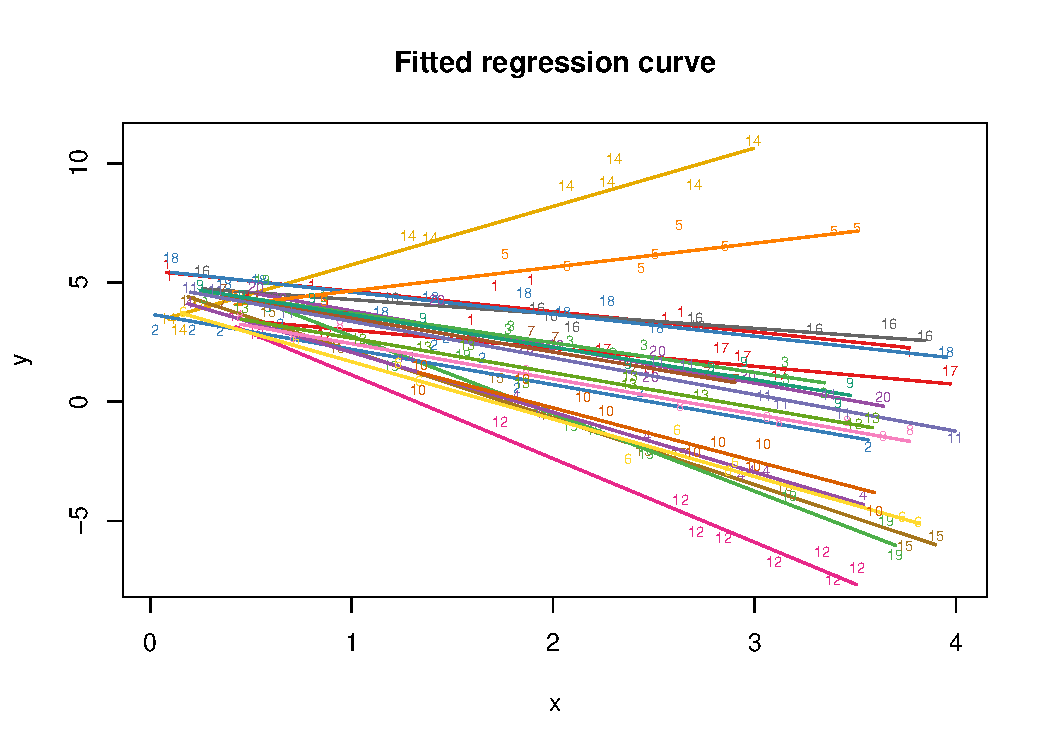
\includegraphics[width=\maxwidth]{figure/iprior_plot-1} 

}

\caption[This is a caption]{This is a caption.}\label{fig:iprior.plot}
\end{figure}


\end{knitrout}

The plot in Figure \ref{fig:iprior.plot} is explained in further detail in \cite{jamil2017}. Notice that I have used a reference to the figure via \verb@\ref{fig:<name-of-chunk>}@. The following shows a side-by-side plot. We can also reference them Figure \ref{fig:iprior.residplot1} and Figure \ref{fig:iprior.residplot2}.

\begin{knitrout}
\definecolor{shadecolor}{rgb}{1, 1, 1}\color{fgcolor}\begin{figure}
\subfloat[The left plot.\label{fig:iprior.residplot1}]{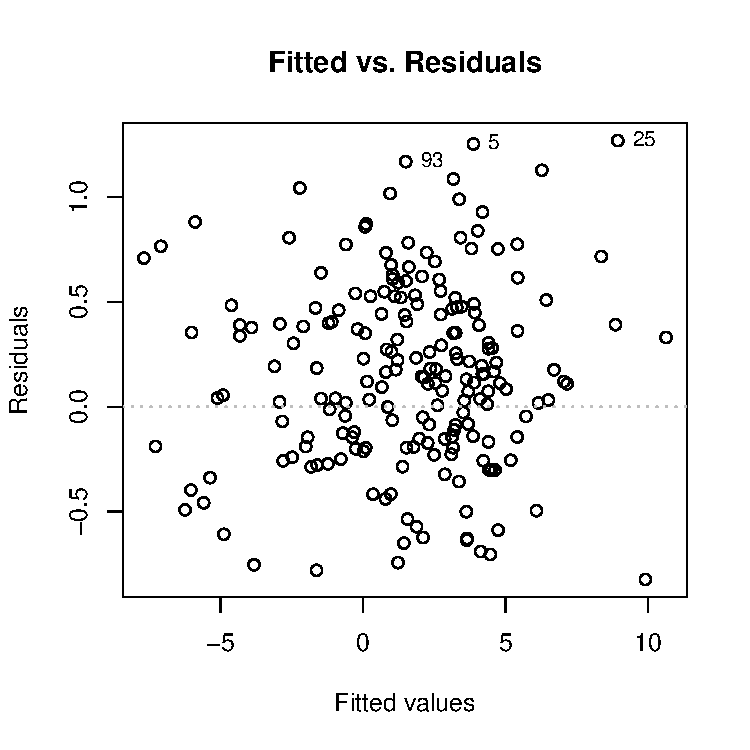
\includegraphics[width=7cm,height=7cm]{figure/iprior_residplot-1} }
\subfloat[And the right one.\label{fig:iprior.residplot2}]{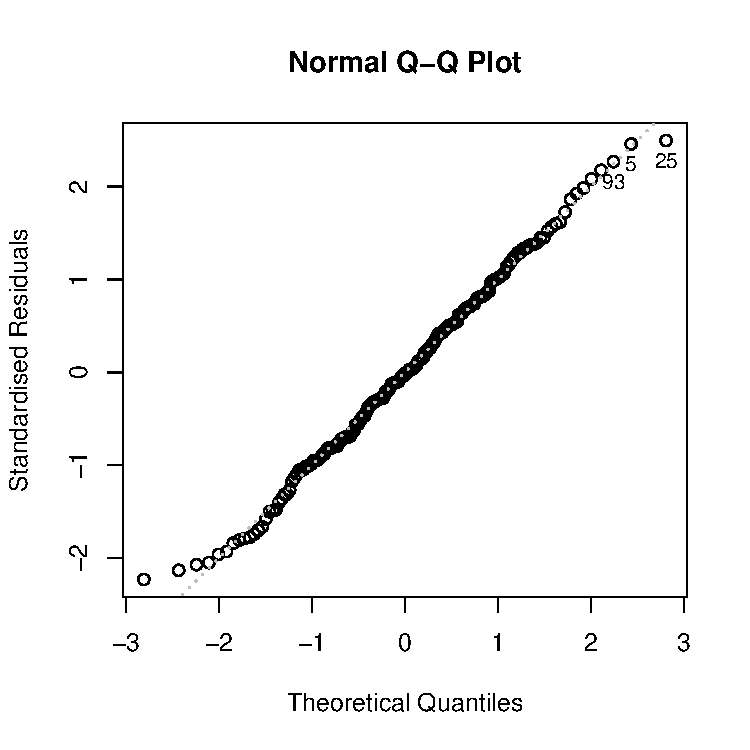
\includegraphics[width=7cm,height=7cm]{figure/iprior_residplot-2} }\caption[Side-by-side plot]{Side-by-side plot}\label{fig:iprior.residplot}
\end{figure}


\end{knitrout}

%%%%%%%%%%%%%%%%%%%%%%%%%%%%%%%%%%%%%%%%%%%%%%%%%%%%%%%%%%%%%%%%%%%%%%%%
%%% REFERENCES %%%%%%%%%%%%%%%%%%%%%%%%%%%%%%%%%%%%%%%%%%%%%%%%%%%%%%%%%
%%%%%%%%%%%%%%%%%%%%%%%%%%%%%%%%%%%%%%%%%%%%%%%%%%%%%%%%%%%%%%%%%%%%%%%%
%\ifstandalone
%\nocite{*}
%\bibliographystyle{apalike}
%\bibliography{haziq}
%\fi

%\end{document}



%%%!TEX root = main.Rnw
%\documentclass[class=article, crop=false]{standalone}
%\ifstandalone
%\usepackage{haziq_article}
%\fi
%\begin{document}



We can include some R code here. Hello

\begin{knitrout}
\definecolor{shadecolor}{rgb}{1, 1, 1}\color{fgcolor}\begin{kframe}
\begin{alltt}
\hlkwd{library}\hlstd{(iprior)}
\hlstd{mod} \hlkwb{<-} \hlkwd{ipriorOptim}\hlstd{(}\hlkwd{kernL}\hlstd{(y} \hlopt{~} \hlstd{.} \hlopt{^} \hlnum{2}\hlstd{,} \hlkwc{data} \hlstd{= simdat))}
\end{alltt}
\begin{verbatim}
## Iteration 0:    Log-likelihood = -491.76134 
## Iteration 1:    Log-likelihood = -452.90519 ........
## Iteration 2:    Log-likelihood = -417.44265 .......
## Iteration 3:    Log-likelihood = -393.65504 .......
## EM NOT CONVERGED!
## 
## Now switching to optim...
## 
## iter   10 value 259.621574
## iter   20 value 255.501753
## final  value 255.454420 
## converged
## 
## Preparing iprior output... DONE.
\end{verbatim}
\begin{alltt}
\hlkwd{print}\hlstd{(mod)}
\end{alltt}
\begin{verbatim}
## 
## Call:
## iprior(formula = y ~ .^2, data = simdat)
## 
## RKHS used: Pearson & Canonical, with multiple scale parameters.
## 
## 
## Parameter estimates:
## (Intercept)     lambda1     lambda2         psi 
##  1.74493392  0.46809945  0.02367604  3.61187777
\end{verbatim}
\end{kframe}
\end{knitrout}
\begin{knitrout}
\definecolor{shadecolor}{rgb}{1, 1, 1}\color{fgcolor}\begin{figure}[h]

{\centering 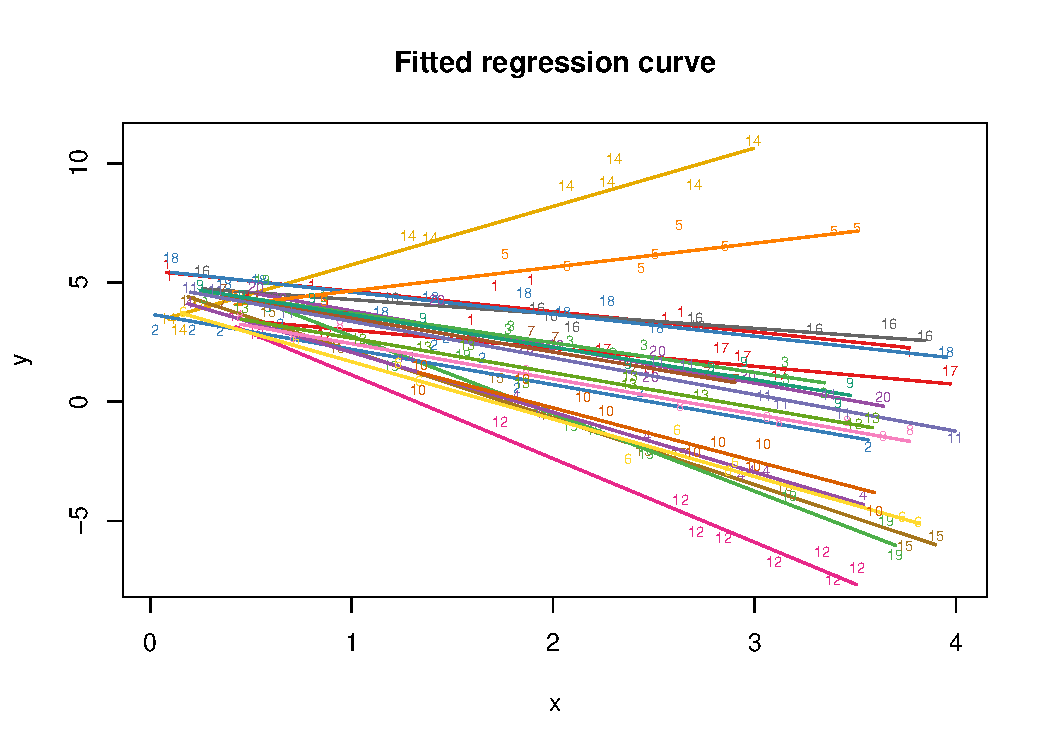
\includegraphics[width=\maxwidth]{figure/iprior_plot-1} 

}

\caption[This is a caption]{This is a caption.}\label{fig:iprior.plot}
\end{figure}


\end{knitrout}

The plot in Figure \ref{fig:iprior.plot} is explained in further detail in \cite{jamil2017}. Notice that I have used a reference to the figure via \verb@\ref{fig:<name-of-chunk>}@. The following shows a side-by-side plot. We can also reference them Figure \ref{fig:iprior.residplot1} and Figure \ref{fig:iprior.residplot2}.

\begin{knitrout}
\definecolor{shadecolor}{rgb}{1, 1, 1}\color{fgcolor}\begin{figure}
\subfloat[The left plot.\label{fig:iprior.residplot1}]{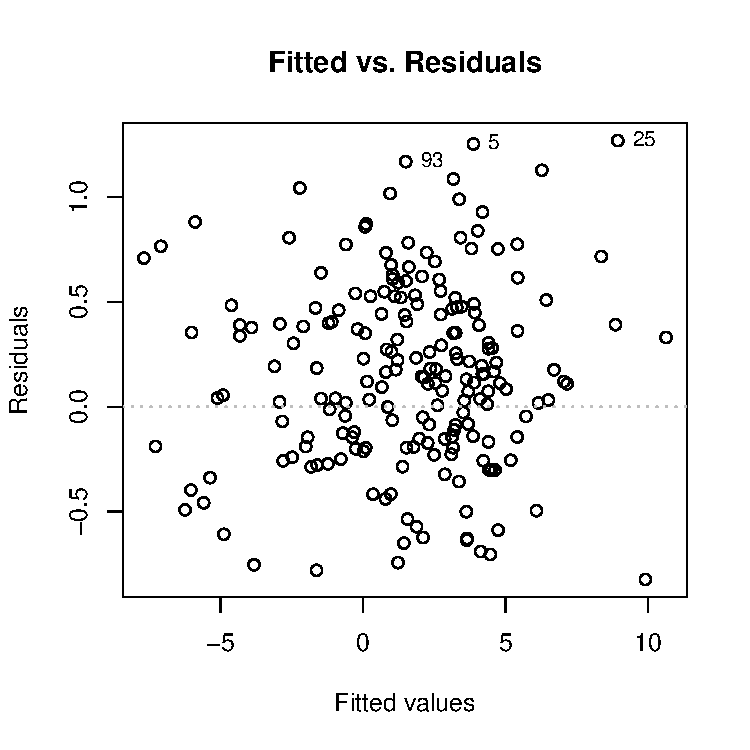
\includegraphics[width=7cm,height=7cm]{figure/iprior_residplot-1} }
\subfloat[And the right one.\label{fig:iprior.residplot2}]{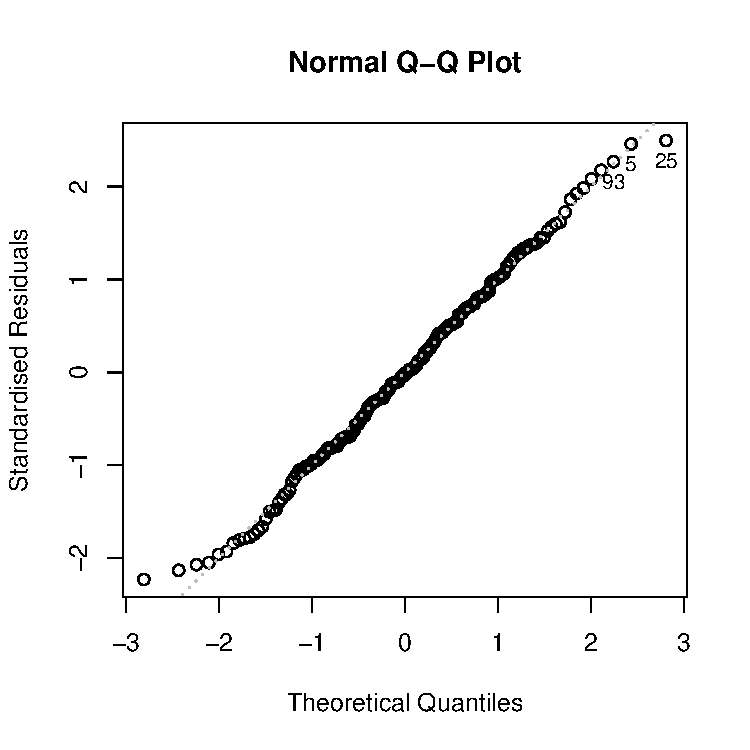
\includegraphics[width=7cm,height=7cm]{figure/iprior_residplot-2} }\caption[Side-by-side plot]{Side-by-side plot}\label{fig:iprior.residplot}
\end{figure}


\end{knitrout}

%%%%%%%%%%%%%%%%%%%%%%%%%%%%%%%%%%%%%%%%%%%%%%%%%%%%%%%%%%%%%%%%%%%%%%%%
%%% REFERENCES %%%%%%%%%%%%%%%%%%%%%%%%%%%%%%%%%%%%%%%%%%%%%%%%%%%%%%%%%
%%%%%%%%%%%%%%%%%%%%%%%%%%%%%%%%%%%%%%%%%%%%%%%%%%%%%%%%%%%%%%%%%%%%%%%%
%\ifstandalone
%\nocite{*}
%\bibliographystyle{apalike}
%\bibliography{haziq}
%\fi

%\end{document}




%%%%%%%%%%%%%%%%%%%%%%%%%%%%%%%%%%%%%%%%%%%%%%%%%%%%%%%%%%%%%%%%%%%%%%%%%%%%%%%%
%%% REFERENCES %%%%%%%%%%%%%%%%%%%%%%%%%%%%%%%%%%%%%%%%%%%%%%%%%%%%%%%%%%%%%%%%%
%%%%%%%%%%%%%%%%%%%%%%%%%%%%%%%%%%%%%%%%%%%%%%%%%%%%%%%%%%%%%%%%%%%%%%%%%%%%%%%%
%\nocite{*}
\bibliographystyle{apalike}
\bibliography{haziq}

%%%%%%%%%%%%%%%%%%%%%%%%%%%%%%%%%%%%%%%%%%%%%%%%%%%%%%%%%%%%%%%%%%%%%%%%%%%%%%%%
%%% APPENDIX %%%%%%%%%%%%%%%%%%%%%%%%%%%%%%%%%%%%%%%%%%%%%%%%%%%%%%%%%%%%%%%%%%%
%%%%%%%%%%%%%%%%%%%%%%%%%%%%%%%%%%%%%%%%%%%%%%%%%%%%%%%%%%%%%%%%%%%%%%%%%%%%%%%%
\appendix
\section{An appendix}
%\documentclass[class=article, crop=false]{standalone}
%\ifstandalone
%\usepackage{haziq_article}
%\fi
%\begin{document}

\lipsum[10-11]

%%%%%%%%%%%%%%%%%%%%%%%%%%%%%%%%%%%%%%%%%%%%%%%%%%%%%%%%%%%%%%%%%%%%%%%%
%%% REFERENCES %%%%%%%%%%%%%%%%%%%%%%%%%%%%%%%%%%%%%%%%%%%%%%%%%%%%%%%%%
%%%%%%%%%%%%%%%%%%%%%%%%%%%%%%%%%%%%%%%%%%%%%%%%%%%%%%%%%%%%%%%%%%%%%%%%
%\ifstandalone
%%\nocite{*}
%\bibliographystyle{apalike}
%\nobibliography{haziq}
%\fi
%
%\end{document}

















\section{Another appendix}
%\documentclass[class=article, crop=false]{standalone}
%\ifstandalone
%\usepackage{haziq_article}
%\fi
%\begin{document}

\lipsum[12-13]

%%%%%%%%%%%%%%%%%%%%%%%%%%%%%%%%%%%%%%%%%%%%%%%%%%%%%%%%%%%%%%%%%%%%%%%%
%%% REFERENCES %%%%%%%%%%%%%%%%%%%%%%%%%%%%%%%%%%%%%%%%%%%%%%%%%%%%%%%%%
%%%%%%%%%%%%%%%%%%%%%%%%%%%%%%%%%%%%%%%%%%%%%%%%%%%%%%%%%%%%%%%%%%%%%%%%
%\ifstandalone
%%\nocite{*}
%\bibliographystyle{apalike}
%\nobibliography{haziq}
%\fi
%
%\end{document}

















%%%%%%%%%%%%%%%%%%%%%%%%%%%%%%%%%%%%%%%%%%%%%%%%%%%%%%%%%%%%%%%%%%%%%%%%%%%%%%%%
\end{document}
%%%%%%%%%%%%%%%%%%%%%%%%%%%%%%%%%%%%%%%%%%%%%%%%%%%%%%%%%%%%%%%%%%%%%%%%%%%%%%%%
